\chapter{Transfer learning}
%\cite{Taylor2009TransferSurvey}.
Transfer learning involves the use of experience gained when learning one or more tasks, to improve the performance on a different but related task. Each task is represented by a Markov Decision Process (MDP).\\  Here, we discuss a framework for transfer methods that can be used for reinforcement learning, closely following \cite{Taylor2009TransferSurvey}.\\

As already said, the transfer of knowledge always happens between one or more source tasks and a target task. First, an appropriate set of tasks must be selected. Afterwards, the transfer learning algorithm must learn how these source tasks are related to the target task. Then, the appropriate knowledge can be transferred.\\

\section{Transfer learning dimensions} % (fold)
\label{sub:transfer_learning_dimensions}
To be able to transfer knowledge, some assumptions must be made about the differences between the source tasks and the target task. This can be for example in the underlying dynamics of the environment, which can make the task harder or easier to solve, or different sets of possible actions at certain states.
These differences define between which type of source and target tasks knowledge can be transferred. The differences between the source task(s) and target task can also make the transfer of knowledge easier or harder, requiring the appropriate guidance by a human or a method that can overcome these differences in case of a fully autonomous transfer learner.\\
Multi-task learning is a special kind of task learning where the problems for the source and target tasks are drawn from the same distribution instead of having arbitrary source and target tasks. More specifically, the transition function is drawn from a fixed distribution of functions. For the mountain car environment, where an underpowered car must be driven up a hill, this may mean for example that the motor of the car differs in power in different tasks.\\

As was stated, first the set of source tasks needs to be selected. Again, this can be done by a human in case of a human-guided scenario. However, the selection may also be done by the agent itself. For example, it can learn multiple source tasks and then use them all for transfer.
Another possibility is to select the source tasks that are the most relevant and lead to highest performance for the target task.
The agent may also just aim to avoid negative transfer, such that the specific selection of source tasks does not worsen the learning performance for the target task.
The agent could also modify the source task(s) such that the transferred knowledge is the most useful in the target task.\\

Instead of just knowing that tasks are related, many methods also need to know how tasks are related, using task mappings. This is necessary to make the knowledge gained on the source tasks useful for the target task. Tasks may differ in state and action variables and the in the semantic meaning of them. In the mountain car environment, one can have a task where the goal is on the opposite side. As such, taking the action \texttt{Left} has a different meaning for these tasks. Actions in the two tasks must be mapped such that their effects are similar.\\
Again, these mappings can be provided by a human or they can be learned by the agent. Note that these mappings may be partial and not every action in the source task is mapped to an action in the target task or vice-versa. For the state space, it is also possible to map the states themselves instead of the state variables.\\
In multi-task learning, states and variables are the same and have the same meaning. Because of this, no task mappings are necessary in multi-task learning.\\

Task learning methods can also differ in the type of knowledge that is transferred between source and target tasks. This knowledge can be for example an action-value function, transitions or policy gradient parameters. For tasks that are closely related, detailed knowledge may be useful. Otherwise, high-level information may result in a better learning performance. The type of knowledge that is transferred can also depend on the type of source and target tasks and on the task mappings.\\

Last, the task learning method may also restrict which reinforcement learning algorithms that can be used. It is possible for example that only a class of reinforcement learning algorithms or only one specific reinforcement learning algorithm can be used with the task learning method or that the algorithm is the same for both the source and target tasks. Ideally, the reinforcement learning algorithms can be chosen freely and may be selected based on the characteristics of the tasks at hand.\\
% section transfer_learning_dimensions (end)

\section{Metrics}
\label{sub:tl_metrics}
Several metrics exist to evaluate the learning performance and solution quality of transfer learning algorithms. Generally, one metric does not give a complete representation of the overall performance of the algorithm. Because of this, often multiple metrics are used.\\
Here we will list the most popular ones:
\begin{itemize}
    \item \textit{Jumpstart}: This is the initial improvement that the target task has over an algorithm that does not use knowledge transfer. However, little to no learning has occurred yet. Because of this, learning performance can't be measured. The metric also does not give an indication about the final performance, i.e.\ the performance after having learned.
    \item \textit{Asymptotic performance}: This is the opposite of \textit{jumpstart} performance and measures the performance improvement after having learned the target task or during the last time steps of the algorithm. However, this is hard to measure because one has to know when the task learning algorithm converged. Furthermore, the task learning algorithm and the algorithm that does not use knowledge transfer may require a different training time in order to converge.
    \item \textit{Total reward}: This is the total reward that the algorithm has accumulated during learning, i.e.\ the area under the learning curve. In case of improvement, this area is bigger than when transfer learning isn't used. This can be achieved when the transfer learning algorithm has a higher learning rate.
    However, convergence is again an issue here. An algorithm that learns slower and thus takes more time to converge may accumulate a higher total reward than a faster algorithm, although the latter may even reach a higher performance. This metric is only useful for tasks that always have the same duration.
    \item \textit{Transfer ratio}: This is the ratio of the total reward improvement that the transfer learning algorithm has over the other algorithm. Because it uses the \textit{total reward} metric, it suffers from the same issues. Furthermore, it is also influenced by the reward structure. For example, an agent always receiving a reward of $+1$ at the end of the episode may result in a different ratio.
    \item \textit{Time to threshold}: This measures the time needed to reach a pre-defined performance. A transfer learning algorithm may need less time to reach this threshold. The threshold needs to be defined manually and depends on the task domain and learning method.
\end{itemize}
A graph with 4 of the 5 metrics is shown in Figure~\ref{fig:TLmetrics}.
\begin{figure}[htb]
    \centering
    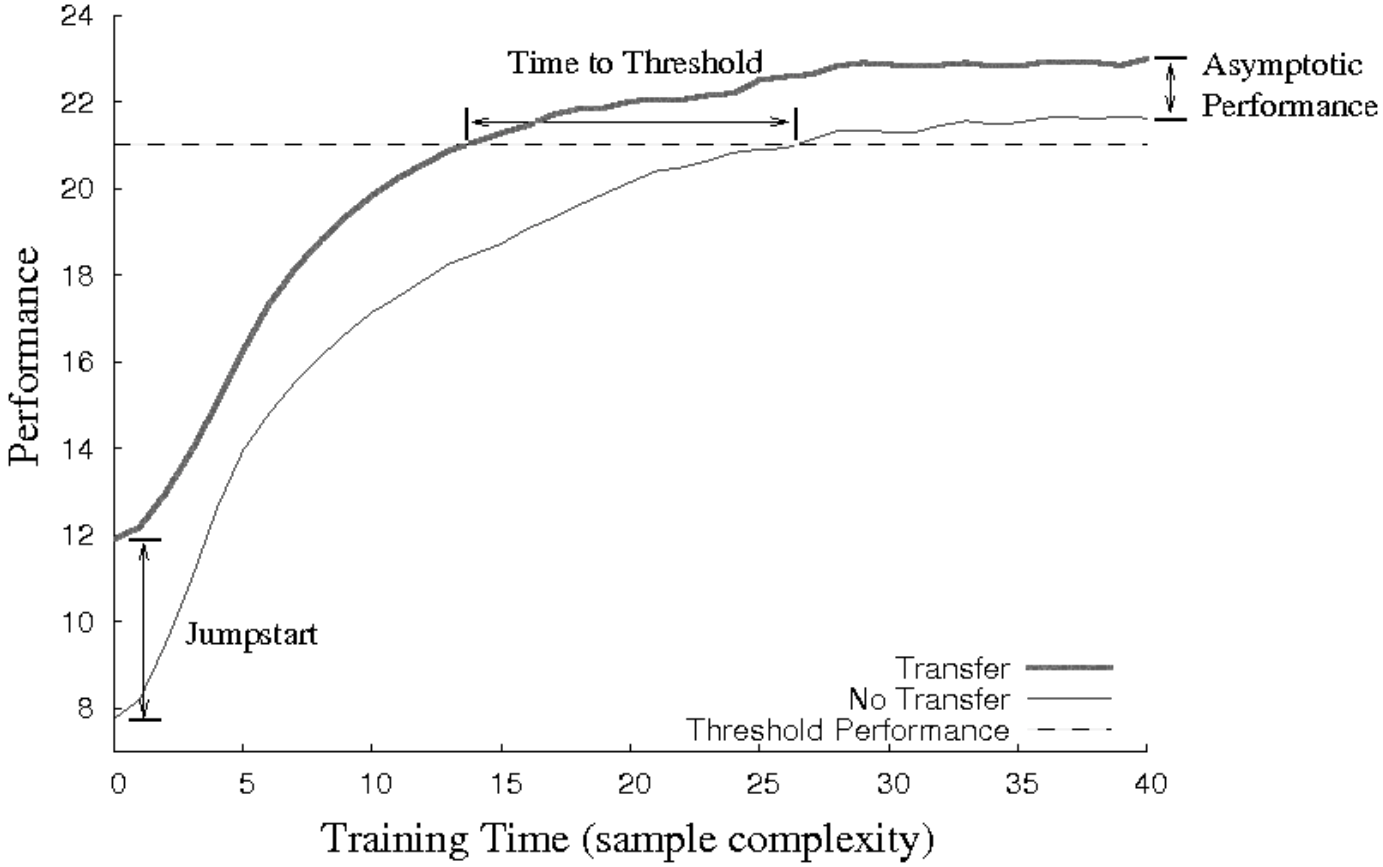
\includegraphics[width=.9\linewidth]{images/tlmetrics.png}
    \caption[Transfer learning metrics]{A graph comparing the \textit{jumpstart}, \textit{time to threshold} and \textit{asymptotic performance} metrics between the algorithm that uses knowledge transfer and the one that does not use it. Note that here the transfer learning algorithm performs better on all three metrics. It can also be seen that the total reward is higher. Source: \cite{Taylor2009TransferSurvey}.}
    \label{fig:TLmetrics}
\end{figure}
Instead of comparing the transfer learning algorithm with an algorithm that does not use knowledge transfer, it is also possible to compare the algorithm with the performance of humans (by averaging their performances).
However, metrics must be chosen carefully such that they do not favor the algorithm or the human and that they cannot be abused.

\section{Related work}
% Types of knowledge that is transferred: Value functions, features extracted from value functions, heuristics, policies
% Different representation types: Graphs, relational representation, tables

% Representation transfer
    % options

% separation in subtasks

% Relational RL

% transferring instances
% transferring advice/preferences
Transfer learning methods for reinforcement learning can be divided into 2 groups: methods that use task mappings and methods that do not.
We will mostly discuss methods that do not use task mappings as our approach also does not use task mappings.\\

In one of the earliest works of transfer learning used for reinforcement learning \parencite{conf/ijcai/SelfridgeSB85}, the transition function was gradually changed as to make the task harder.
A \emph{cart-pole} task was used where the pole was long and light at first, but was made shorter and heavier over time.
The total time spent learning on the sequence of gradually modified tasks was shorter than when trying to solve the hardest task directly.\\

Later work was generally focused on transferring from one source task to a target task, while in recent research, most of the times a more general scenario with possibly multiple source tasks is considered.
The approaches that we will further discuss mostly focus on transferring from multiple source tasks instead of just one.
We do this because our approach also allows the use of multiple source tasks.
Furthermore, the  discussed algorithms that can use multiple source tasks generally also allow just one source task from which to transfer knowledge.\\

One approach, presented in \cite{lazaric2008transfer}, is to transfer transitions (also called \textit{instances} or \textit{samples}) gathered from the source tasks to the target task.
However, transitions may not be useful if the target tasks differs too much from the source tasks.
To solve this, transitions from source tasks are chosen based on the similarity of these tasks to the target task.
After having trained on the source tasks and collected transitions, we also collect a few transitions from the target task.
The similarity between a source task and the target task is then the probability that the transitions of the target task were generated by an approximated model of the source task.

\cite{Ammar2014} also focus on the problem of selecting the appropriate source tasks from which to transfer knowledge.
Here, however, a Restricted Boltzmann Machine \parencite{Smolensky1986} is used in order to generate a model of a source tasks that yields features that are relevant for characterizing the task.
The model, generated using transitions of the source task, then tries to reconstruct samples of the target task.
The similarity of a source and target task can then be assessed using the difference of the reconstructed transitions and the real transitions of the target task.
Note however that the state and action spaces of the source tasks and target task needs to be the same.\\

Another possibility is to transfer a representation, for example by transferring features extracted from the states. In this case, characteristics are inferred from multiple source tasks.
In \cite{Bernstein99reusingold}, policies are averaged and can be applied for $n$ time steps on all states.
This combination of a policy, time steps to execute and states is called an option.
The reasoning is that actions that are used a lot in a state in source tasks may also be useful in the target task. In \cite{perkins1999using}, these options are provided on beforehand.
The agent then learns a single action-value function over these options using all the source tasks.
These options along with the action-value function can then be transferred and used for the target task.\\

Instead of using a single policy or action-value function, one can also collect a library of policies and select one to use probabilistically, depending on the expected reward. This approach is presented in \cite{fernandez2006probabilistic,fernandez2013learning}. At every time step, the algorithm can choose to use one of the source task policies, use the current best target task policy or to randomly explore. As the probabilities depend on the gained rewards, after some time more useful policies are exploited more often. This method only works however for tasks where only the goal state in a maze is different.\\

In \cite{conf/cira/TanakaY03} action-value functions are transferred instead of policies and statistics about those functions are exploited.
More specifically, the average and standard deviation of the value each state-action pair is calculated.
In the target task, the action-value function for each state-action pair is then instantiated to the average for that pair for the source tasks.
The standard deviation is used in order to prioritize updates for state-action pairs that are far from the average.
Besides this, states-action pairs that fluctuate often within an episode are also prioritized.\\

\cite{journals/ml/FosterD02} try to extract sub-tasks across multiple source tasks.
Optimal policies are then learned for each of these sub-tasks and pieced together.
In this case, the environment was a maze and tasks differ in their goal in the maze.
Value functions can then be learned on parts of the maze.
Less learning for the target task is then required because most of the already learned sub-tasks can also be used for the target task.\\

Most methods focus on problems with a discrete state and action space. However, other methods exist that can be applied on problems with a continuous state and action space.
Here, function approximation is always required. \cite{walsh2006transferring} group states encountered in the source tasks and treat them as being one and the same state.
This abstraction along with the value function learned on this abstraction can then be transferred and used for learning the target task.\\
\cite{lazaric2008knowledge} also groups states of the source tasks, but does this by adjusting parameters of a function approximator to build features.
Only a small set of features are searched while still being able to learn useful value functions. The learning process for the tasks is executed in parallel.
Again, after learning the source tasks, the parameters of the function approximator and the value functions are transferred.

2 other approaches use a hierarchical Bayesian model. They use this to find parameters that make up the dynamics and reward function of a problem. In \cite{sunmola2006model}, transitions of source tasks are used as a prior to find parameters for models.
After getting transitions from the target task, the most probable model for the target task transitions is transferred and used.\\
\cite{conf/icml/WilsonFRT07} use a similar approach, but they do not make a distinction between source and target tasks. Instead, problems (MDPs) are executed sequentially and models are built using an already acquired set of transitions and models of previous tasks.\\

In \cite{Isele2016UsingLearning}, a multi-task learning method is presented that learns tasks simultaneously by using a predefined description for each task.
When a new task arrives along with its features, obtained from its task descriptor, a policy can be generated that immediately results in a good performance, even though the algorithm was not applied on that task before and the task descriptor, task order and task distribution were not known on beforehand. This is called \textit{zero-shot learning}.
As such, knowledge transfer can take place without the need of training data to identify relationships across tasks.
For each subsequent task, the policy and feature vector are iteratively improved.\\
%factorization: ontbinding in factoren: bijv. 15=3*5
First, it is assumed that the policy parameters for every task $t$ can be factorized using a shared knowledge base $L \in \mathbb{R}^{d \times k}$: $\theta^{(t)} = Ls^{(t)}$. $s^{(t)} \in \mathbb{R}^{(k)}$ are the sparse coefficients over the basis, i.e.\ the latent representation of the policy's parameters for task $t$. $L$ is able to capture relationships among policies as this is used to compute every policy, whereas there is a sparse representation for computed for each task separately.\\
The features of the task are obtained by (possibly non-linear) feature extractors applied on the descriptor of the task: $\phi(m^{(t)}) \in \mathbb{R}^{d_m}$.
These features can also be linearly factorized using another shared knowledge base $D \in \mathbb{R}^{d_m \times k}$: $\phi(m^{(t)}) = Ds^{(t)}$, where the same sparse representation is used as the one used to compute the policy.
Both knowledge bases provide information about the task and because of this they share the same coefficient vectors $S$.
We then use coupled dictionary optimization techniques from the sparse coding literature to optimize these dictionaries.
The dictionaries updated iteratively based on trajectories sampled from the current task.\\
When a new task arrives along with its task descriptor, we search for the coefficients $s^{(t_{new})}$ that minimize the difference between the extracted features and the reconstruction of it using the shared knowledge base $D$.
Using these coefficients, we can compute the policy parameters using $\theta^{(t_{new})} = Ls^{(t_{new})}$. Afterwards, we can iterate again to improve the sparse representation and the knowledge bases.\\

Together with the interest in deep reinforcement learning \parencite{Mnih2015Human-levelLearning,Mnih2016AsynchronousLearning}, the interest in its application to transfer learning also grows.
In \cite{DBLP:journals/corr/ParisottoBS15}, the algorithm, Actor-Mimic Network (AMN), learns the $Q$ function for source tasks from an expert for each specific task (in this paper a DQN that was trained until convergence).
Note that only one set of parameters (and thus one artificial neural network) is used to learn on all the source tasks.
As can be seen, this is supervised learning (more specifically regression) with the output of the expert's network as target value.
As input, both the expert and the AMN can be used to sample trajectories.
Besides mimicking using the expert's output, the AMN also tries to mimic the hidden layer activations of the expert's network.
This is done by adding a loss in function of the difference between the hidden layer activations of the expert network and the activations of the AMN.
Intuitively, this gives insight to the AMN, also called to student, why it should act in a specific way, in addition to telling how it should act.
After learning for a pre-determined number of frames on each task, the weights of the AMN are transferred to a DQN and the algorithm trains on an unseen target task.
Note that each task is a different kind of task here (i.e.\ the state space, action space, transition function and reward function can be different).
However, the algorithm can also be applied to tasks with the same state and action space.

% Progressive neural networks
In contrast to the previous algorithm, Progressive Neural Networks \parencite{Rusu2016} use A3C to learn tasks.
However, the focus here is on avoiding catastrophic forgetting, which causes previously learned weights to be overwritten when there is a different distribution in the data.
In this case, this means that we are learning a different task.
To solve this problem, a different set of artificial neural network weights is used for each task.
Knowledge is transferred using lateral connections from neurons of artificial neural networks used for previously learned tasks.\\
After a task is learned, the weights of the used artificial neural networks are kept fixed.
When a new task has to be learned, a new artificial neural network is instantiated, with each neuron being both the result of its own knowledge and that of previous tasks:
\begin{equation}
    h^{(k)}_i = f \left ( W^{(k)}_i h^{(k)}_{i-1} + \sum_{j<k} U^{(k:j)}_i h^{(j)}_{i-1} \right )
\end{equation}
Where $h^{(k)}_i$ is the output for layer $i$ of task $k$, $f$ is an element-wise activation function, $W^{(k)}_i$ is the weight vector for layer $i$ of task $k$ and $U^{(k:j)}_i$ are the lateral connections from layer $i-1$ of task $j$ to layer $i$ of task $k$.\\
The algorithm learns both its own weights and its lateral connections from the previous tasks.
Thus, it can decide which knowledge from previous tasks is useful.
However, it is not necessary to use this knowledge from previous tasks, as they may not be similar enough for the current task.
The task also cannot be influenced by future tasks, as it has no lateral connections from them.\\
A limitation of this algorithm is that a large amount of memory is required because each task has its own set of weights. It is also reported that only a fraction of those weights is utilized.
